\section{Quantum Modulations}
    As in a classical system, it is possible to define the concept of modulation for a 
    quantum communication system. The transmitted information will be associated to a 
    quantum state of the electromagnetic field, so it can be transmitted on the communication 
    channel.

    It is possible to think about the quantum transmitter as in figure \ref{fig:2.1}. The bit source
    emits a bit sequence $a[n]$, the serial-parallel converter parallelizes a group of $l$-bit (where
    if $L$ is the number of quantum states, $l=\log_2(L)$) and sends them to the quantum modulator.
    This latter associates one quantum state to every group of bit. The operation of quantum state 
    creation, in real cases, is affected by noise.

    The sequence of operations is very close to a classical transmitter: the main difference is that
    the modulator maps the bits into quantum states instead of classical modulation. Therefore, it is 
    possible to achieve the quantum equivalent of classical modulation, with several states. After 
    that, the impact on performance can be tested.
    This thesis only considers and assesses the binary cases, in the OOK and BPSK 
    configuration.
    
    \subsection{OOK modulations}
        The OOK (on-off keying) is the most simple possible configuration for a communication system.
        The quantum implementation of that is realized associating the low-energy state to the 
        ground state $\ket{0}$ and the high-energy state to another state. It is important to
        consider that the physical realization of these states are not free-noise; this issue will be
        considered using noisy states \ref{eq:2.1.1}.
        \begin{equation}\begin{split}
            \Operator{\varXi}_0 &= \Operator{\varXi}_{\mathrm{th}}\\
            \Operator{\varXi}_1 &= \Operator{\varXi}_{\mathrm{th}}(\mu)
            \label{eq:2.1.1}
        \end{split}\end{equation}
        In the equation \ref{eq:2.1.1}, the high-energy state is associated to a coherent state. This 
        configuration has been widely analyzed in \cite{helstrom1,helstrom2,coherentComm1,coherentComm2,
        coherentComm3,coherentComm4} but this is not the only possible way. The use of PACS states 
        $\Operator{\varXi}_{\mathrm{th}}^{(k)}(\mu)$ is analyzed in \cite{PACSDisc,tesiGuerrini}; the use of PASS are briefly
        assessed in the following chapter of this thesis.

    \subsection{BPSK modulations}
        \begin{figure}[t]
            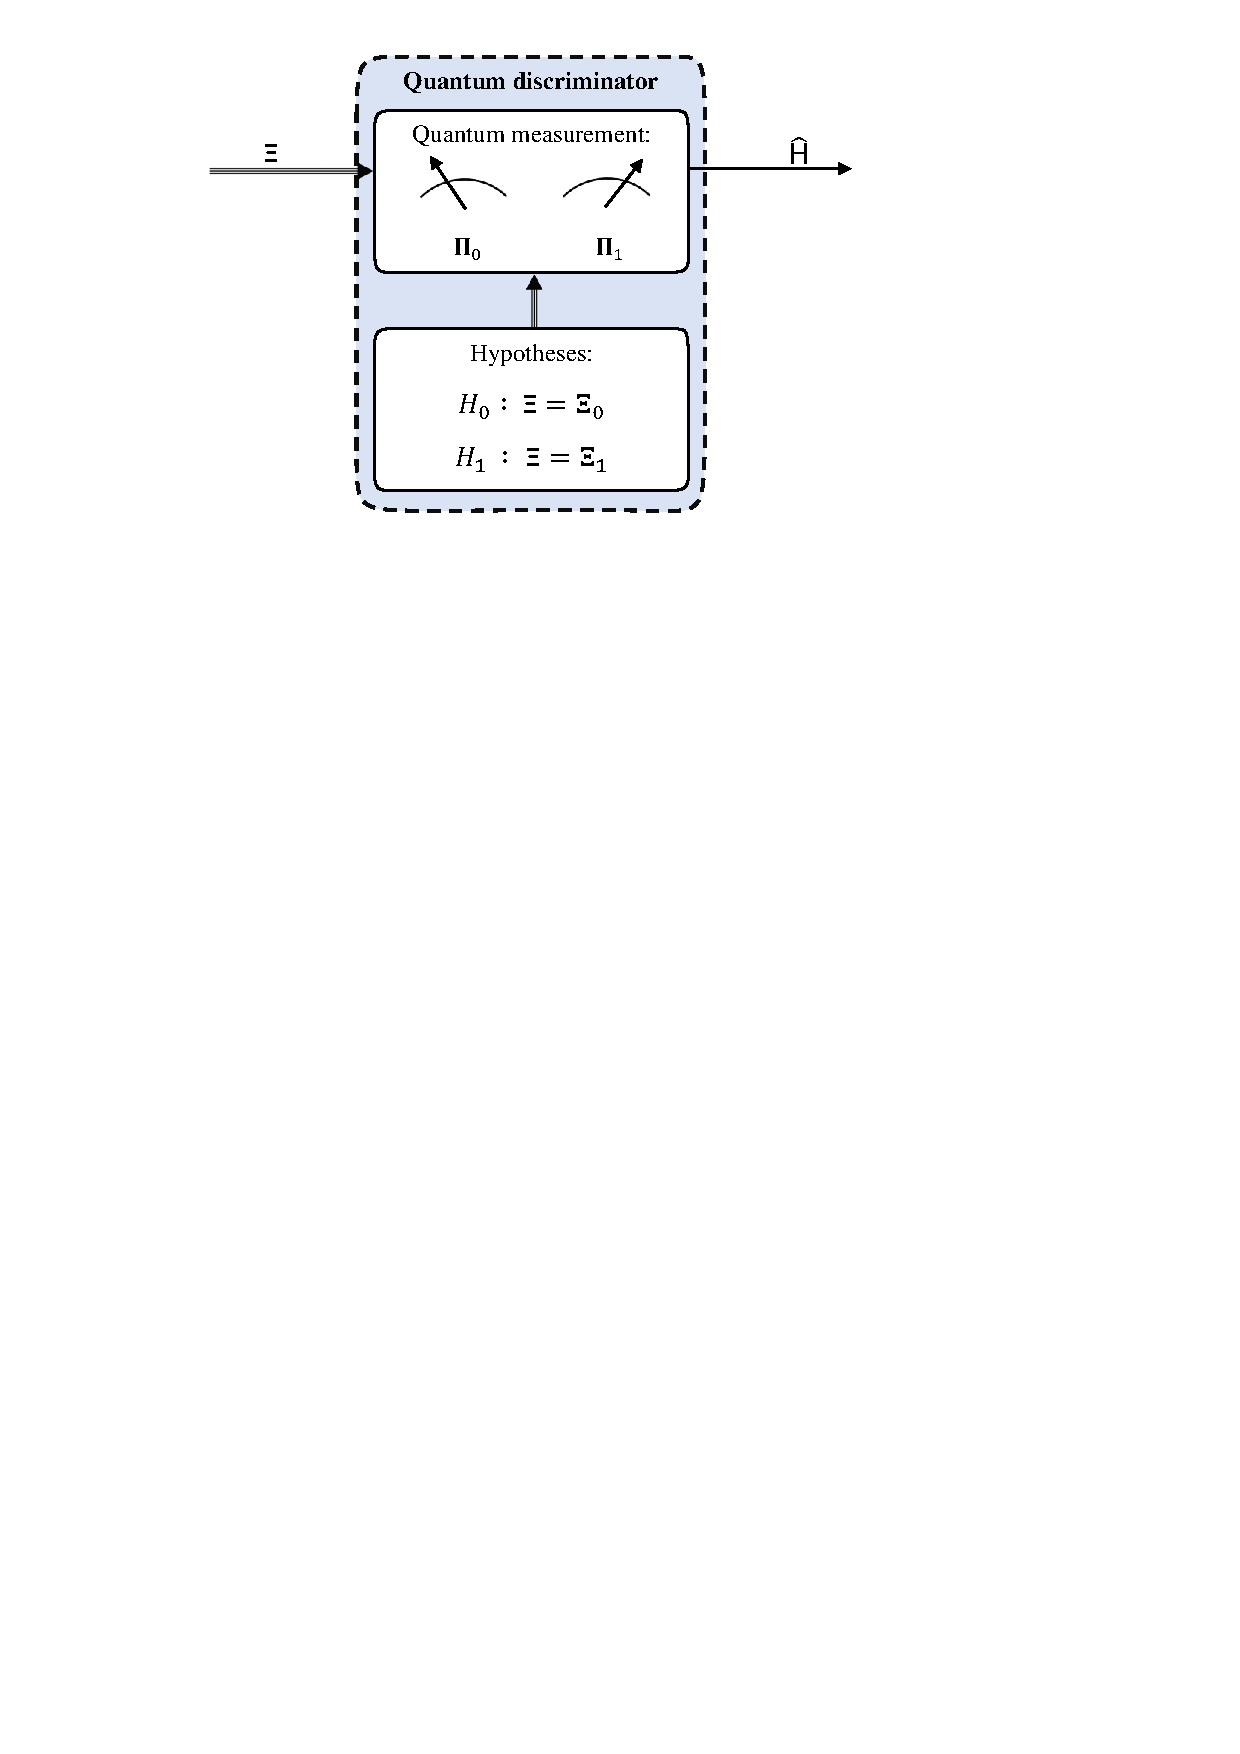
\includegraphics[width=1\textwidth]{fig2.1.pdf}
            \caption{Block diagram of a quantum transmitter.}
            \label{fig:2.1}
        \end{figure}
        BPSK quantum systems are implemented using two states with opposite amplitude, like
        \begin{equation}\begin{split}
            \Operator{\varXi}_0 &= \Operator{\varXi}_{\mathrm{th}}(-\mu)\\
            \Operator{\varXi}_1 &= \Operator{\varXi}_{\mathrm{th}}(\mu).
            \label{eq:2.1.2}
        \end{split}\end{equation}
        There is no guarantee that the use of a BPSK solution in  a quantum system will 
        improve its performance. The effect depends on which are the used states. In the next chapter some 
        configuration are assessed.
